\documentclass{article}
\usepackage{bm}
\usepackage{amsmath}
\usepackage{amssymb}
\usepackage{listings}  
\usepackage{graphicx}
\usepackage{subcaption}
\usepackage{mdwlist}
\usepackage[colorlinks=true]{hyperref}
\usepackage{geometry}
\geometry{margin=1in}
\geometry{headheight=2in}
\geometry{top=2in}
\usepackage{palatino}
%\renewcommand{\rmdefault}{palatino}
\usepackage{fancyhdr}
%\pagestyle{fancy}
\rhead{}
\lhead{}
\chead{%
  {\vbox{%
      \vspace{2mm}
      \large
      Embedded Systems and Applications 4190.303C \hfill
\\
      Seoul National University
      \\[4mm]
      Homework \#(\textbf{2})\\
      \textbf{Oh Hyun Seok}\\
	\textbf{2014-13485}
    }
  }
}



\setlength{\marginparwidth}{2.15cm}


\begin{document}
\pagestyle{fancy}

%% Q1
\section{Analyze Pascal VOC 2012(only segmentation)}
Segmentation: Generating pixel-wise segmentations giving the class of the object visible at each pixel, or "background" otherwise.
\subsection{Class names}
The twenty object classes that have been selected are:\\
Person: person\\
Animal: bird, cat, cow, dog, horse, sheep\\
Vehicle: aeroplane, bicycle, boat, bus, car, motorbike, train\\
Indoor: bottle, chair, dining table, potted plant, sofa, tv/monitor
\subsection{Image size}
Images in dataset can have diverse sizes. They all have 3 channels (RGB) in common, but their width and height varies according to image. Their class segmentation and object segmentation images also have corresponding diverse image sizes. For instance, for segmentation train dataset there are 244 different image sizes. Their width varies from 112 pixels to 500 pixels, and height varies from 246 to 500 pixels.
\subsection{Number of images of each dataset}
train : 1464 images listed at VOC2012/ImageSets/Segmentation/train.txt\\
val : 1449 images listed at VOC2012/ImageSets/Segmentation/val.txt\\
trainval : 2913 images listed at VOC2012/ImageSets/Segmentation/trainval.txt\\
trainaug : dataset from VOC2012 are augmented with \href{https://www.dropbox.com/s/oeu149j8qtbs1x0/SegmentationClassAug.zip?dl=0}{SegmentationClassAug dataset} made by \href{https://github.com/DrSleep/tensorflow-deeplab-resnet}{someone} from \href{http://home.bharathh.info/pubs/codes/SBD/download.html}{Semantic Boundaries Dataset (SBD)} leads to 10582 images for training.\\
\subsection{Meaning of outline}
On images at VOC2012/SegmentationObjects or VOC2012/SegmentationClass, you can see that images have white outlines in common. These outlines are used to calculate IoU which is common metric for segmentation evaluation. Also it indicates acceptable error of segmentation. When we compare ground truth image and our segmented image, our image should segment similar to ground truth image, with range of segmentation error on outline allowed. Segmented pixel covered by outline is masked and excluded on evaluation. I got this idea from PASCAL VOC 2012 devkit VOCevalseg.m file. \\
%% Q2
\section{Evaluation Metric: mIoU}
For each class, IoU metric is intersection of groundtruth segmentation area and our segmentation area divided by union of a class ground truth segmentation area and out segmentation area. This is equal to the number of correctly classified pixels divided by (number of correctly classified pixels + number of wrongly classified pixel + number of wrongly not classified pixel), equivalent to true positive divided by (true positive+ false positive + false negative). Mean IoU metric, also called mIoU is evaluating IoU under accumulated pixels through images.
\subsection{How to calculate mIoU with outline}
for a ground truth segmentation image "gtim", outlines have value 255 and segmented pixels which are not outline pixels have value range from 0(background) to 20 (equal to number of classes).  Predicted segmentation image "resim" does not have outline pixels, but equal range of segmented pixels. We define "sumim" as $(1 + \text{gtim}) + (\text{resim} * (\text{number of classes} + 1))$, and make a histogram "hs" sized $(\text{number of classes} + 1)^2$ of sumim according to pixel value of sumim, since $1 \le (1+\text{gtim}[i,j]) + (\text{resim}[i,j] * (\text{number of classes} + 1)) \le (\text{number of classes} + 1)^2$. In this case, the number of intersections of gtim and resim in class k $(0 \le k \le \text{number of classes})$ equals to $\text{hs}[k,k]$. Also number of pixels of gtim in class k is $\text{hs}[k,:]$, and and resim in class k is $\text{hs}[:,k]$. So union of pixels of gtim and resim in class k is $\text{hs}[k,:] + \text{hs}[:,k] - \text{hs}[k,k]$. We can calculate IoU of class k on one segmentation as 
\begin{align*}
\text{IoU}[k[ = \frac{\text{hs}[k,k]}{ \text{hs}[k,:] + \text{hs}[:,k] - \text{hs}[k,k]}
\end{align*}
 Good thing is that we can accumulate hs for each images to calculate mean IoU for multiple images. At VOCevalseg.m file, hs for each image is accumulated in "confcounts" identifier, and mean IoU for each class k is calculated as 
\begin{align*}
\text{accuracies}[k] = \frac{\text{confcounts}[k,k]}{\text{confcounts}[k,:] + \text{confcounts}[:,k] - \text{confcounts}[k,k]} * 100
\end{align*} \\
On calculating hs, we calculate gtim $<$ 255 which returns boolean gtim-sized array falsifying only outlines in gtim. Then we mask sumim with it before we make hs out of it,  which means that segmentation error on outline area are acceptable.
%%Q3
\section{Analyze DeepLab v3+}
The architecture on Fig.1. uses Atrous convolution initially to extract low-level features. The feature map from atrous convolution goes through 1x1 convolution to become low-level features. After that, it uses layer structure similar to inception module. But it has difference from inception module in using atrous convolution of 3x3 conv rate 6,12,18 and Image pooling instead of normal convolution 3x3 or 5x5 and max pooling. This is called Atrous Spatial Pyramid Pooling. It concatenates feature maps just like Inception module, then applies 1x1 convolution for effective representation. This feature map is high level features.\\
On decoder level, high level features are upsampled by 4 and concatenated by low level features. Concatenated multilevel features go through 3x3 convolution and upsampled by 4 to form a per-pixel image segmentation prediction.
\subsection{Discuss why DeepLab v3+ gets better accuracy than other segmentation networks}
Atrous convolution is based on original convolution, but has a property called rate. it gets value for every stride of rate from input and multiply with kernel. original convolution could be seen as atrous convolution of rate 1. Using atrous convolution, we can increase the size of receptive field without increasing parameters or computations as in original convolution.  With larger receptive field, we have larger field-of-view. We can obtain larger field of view also from down sampling, but down sampling decreases the resolution and causes loss of information. atrous convolution can acquire very large field of view using high rate without loss of information and resolution. On image segmentation, decision is done in pixel basis, so gathering context information for each pixel much as possible is very important, and larger field of view gathers context information better. Compared to other segmentation networks using max pooling, frequent upsampling and original convolution, Deeplab v3+ uses atrous convolution majorly and uses less number of upsampling due to less pooling. Therefore Deeplab v3+ can attain much larger field of view and gather more context information in one pixel without losing information or decreasing resolution. This might be the reason Deeplab v3+ gets better accuracy than other segmentation networks.\\
\begin{figure}
\includegraphics[width=\linewidth]{deeplabv3.png}
\caption{deeplabv3 architecture}
\end{figure}
\subsection{Run on a few images on two networks}
I have run images including one of 6 classes through both MobileNet V2 (mobilenetv2 \textunderscore coco\textunderscore voctrainaug) and Xception(xception\textunderscore coco\textunderscore voctrainaug) base. I have majorly posted images which failed to correctly segment images. From results, classes which are expected good accuracy seems to be segmented quite well, but both models failed to correctly segment people from image of crowds. Classes which are expected bad accuracy seems to be segmented not quite well, especially for dining table class. Figure 2 and 3 came from MobileNet V2, Figure 4 and 5 came from Xception.
%%MobileNet
\begin{figure}[h!]
\begin{subfigure}[b]{1.0\textwidth}
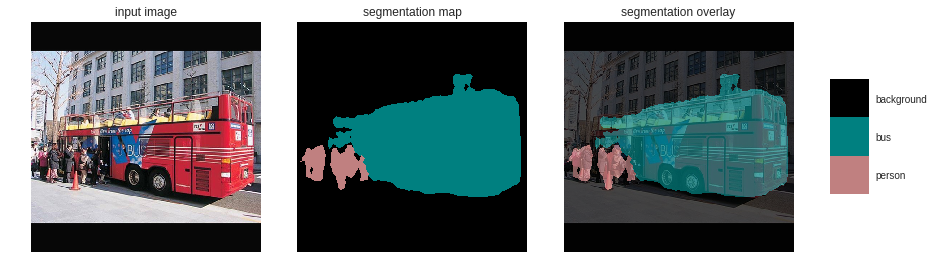
\includegraphics[width=\linewidth]{bus1.png}
\caption{bus}
\end{subfigure}
\begin{subfigure}[b]{1.0\textwidth}
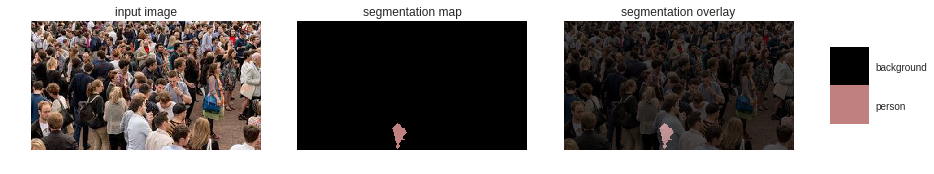
\includegraphics[width=\linewidth]{people.png}
\caption{people}
\end{subfigure}
\begin{subfigure}[b]{1.0\textwidth}
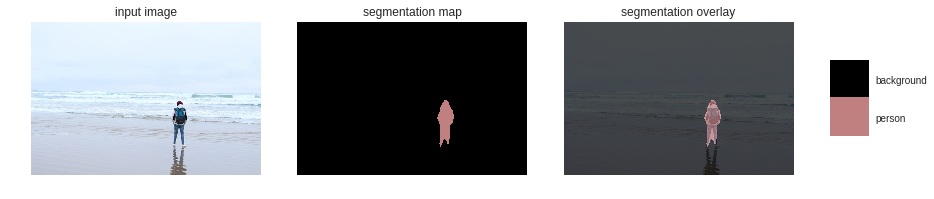
\includegraphics[width=\linewidth]{person.png}
\caption{person}
\end{subfigure}
\begin{subfigure}[b]{1.0\textwidth}
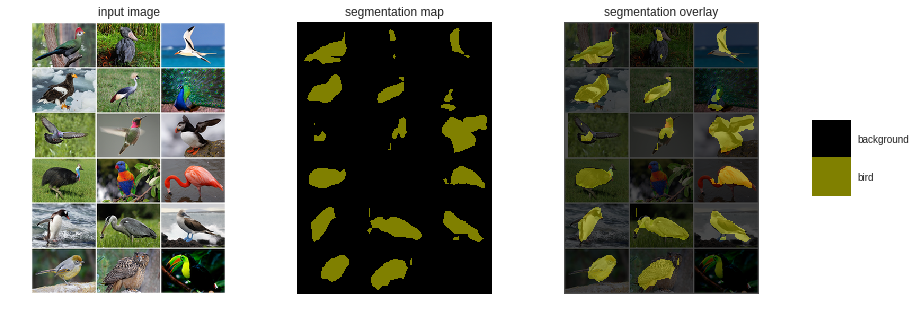
\includegraphics[width=\linewidth]{birds.png}
\caption{birds}
\end{subfigure}
\caption{MobileNet v2 Good Accuracy}
\end{figure}
\begin{figure}[h!]
\begin{subfigure}[b]{1.0\textwidth}
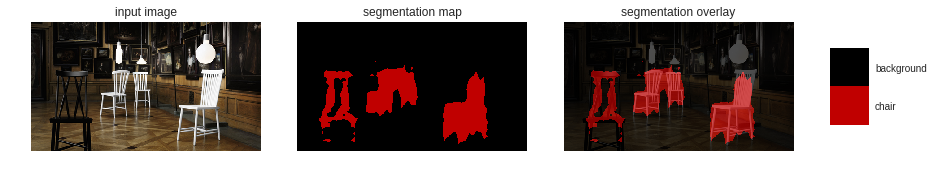
\includegraphics[width=\linewidth]{chair.png}
\caption{chair}
\end{subfigure}
\begin{subfigure}[b]{1.0\textwidth}
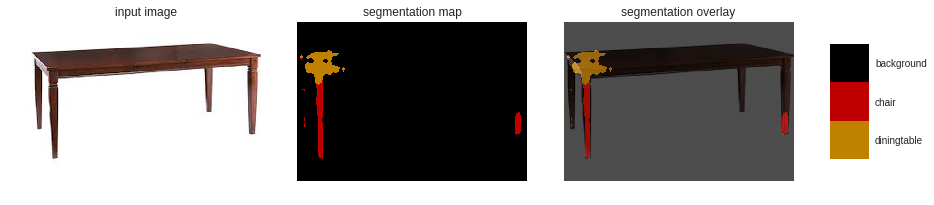
\includegraphics[width=\linewidth]{dining_table2.png}
\caption{dining table}
\end{subfigure}
\begin{subfigure}[b]{1.0\textwidth}
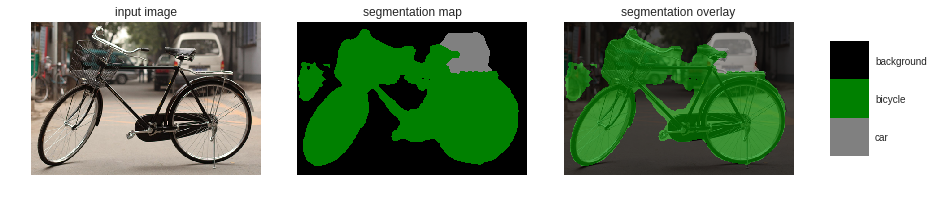
\includegraphics[width=\linewidth]{bicycle1.png}
\caption{bicycle}
\end{subfigure}
\begin{subfigure}[b]{1.0\textwidth}
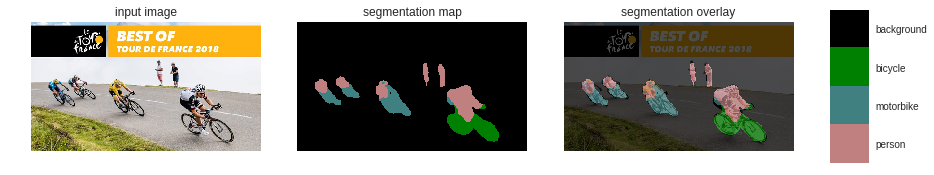
\includegraphics[width=\linewidth]{bicycle2.png}
\caption{bicycles}
\end{subfigure}
\caption{MobileNet v2 Bad Accuracy}
\end{figure}
%% Xception 
\begin{figure}[h!]
\begin{subfigure}[b]{1.0\textwidth}
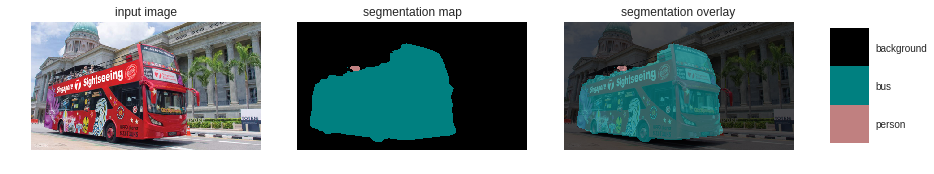
\includegraphics[width=\linewidth]{bus2_xception.png}
\caption{bus}
\end{subfigure}
\begin{subfigure}[b]{1.0\textwidth}
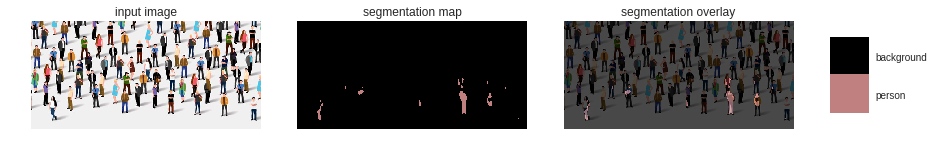
\includegraphics[width=\linewidth]{people_xception.png}
\caption{people}
\end{subfigure}
\begin{subfigure}[b]{1.0\textwidth}
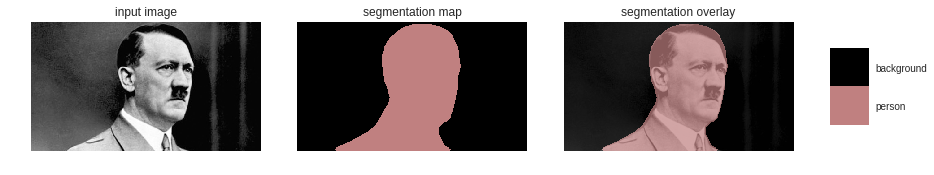
\includegraphics[width=\linewidth]{person_xception.png}
\caption{person}
\end{subfigure}
\begin{subfigure}[b]{1.0\textwidth}
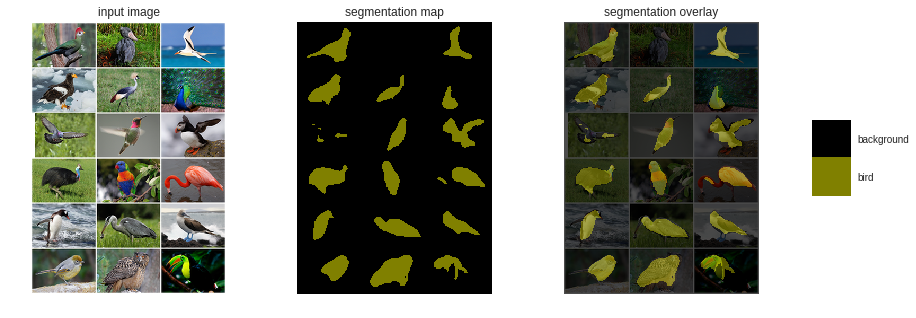
\includegraphics[width=\linewidth]{birds_xception.png}
\caption{birds}
\end{subfigure}
\caption{Xception Good Accuracy}
\end{figure}
\begin{figure}[h!]
\begin{subfigure}[b]{1.0\textwidth}
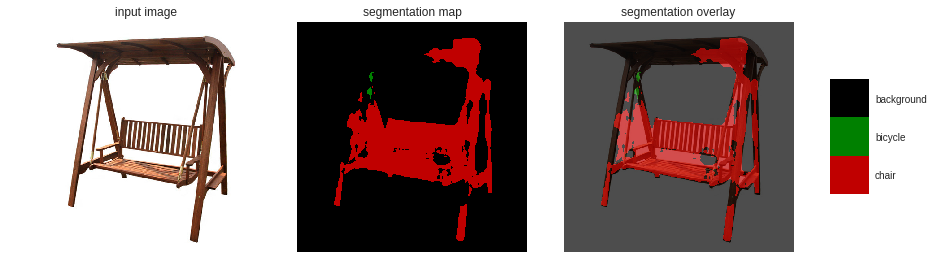
\includegraphics[width=\linewidth]{chair2_xception.png}
\caption{chair}
\end{subfigure}
\begin{subfigure}[b]{1.0\textwidth}
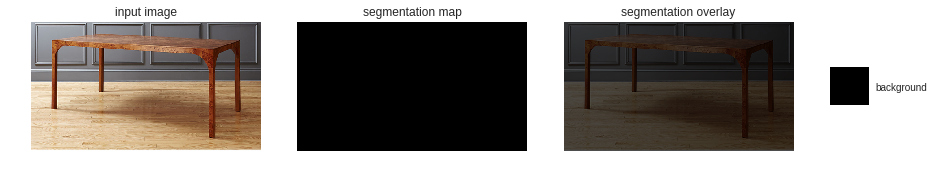
\includegraphics[width=\linewidth]{dining_table1_xception.png}
\caption{dining table}
\end{subfigure}
\begin{subfigure}[b]{1.0\textwidth}
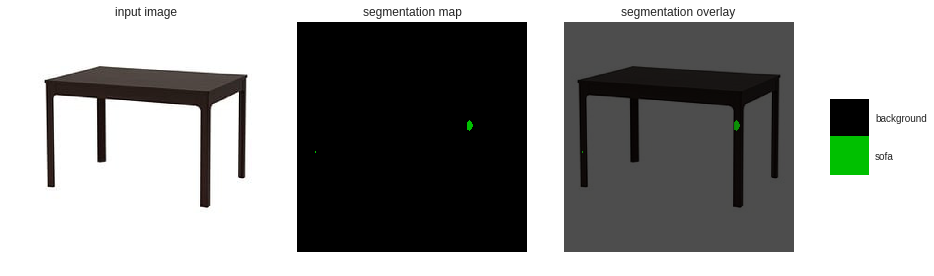
\includegraphics[width=\linewidth]{dining_table3_xception.png}
\caption{dining table}
\end{subfigure}
\begin{subfigure}[b]{1.0\textwidth}
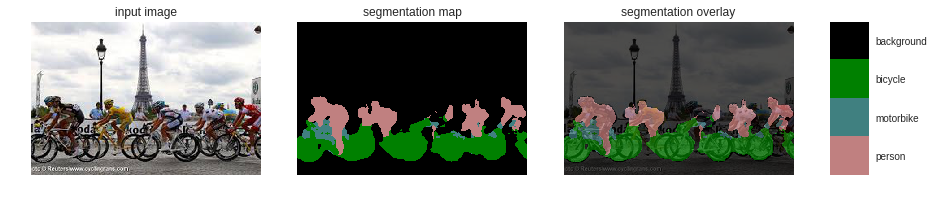
\includegraphics[width=\linewidth]{bicycle1_xception.png}
\caption{bicycles}
\end{subfigure}
\caption{Xception Bad Accuracy}
\end{figure}
\end{document}
